%This document describes the master thesis work done at \gls{rsn} in Lule�, an institute dedicated to the development of data center technology in northern Sweden. At the time of writing their main areas of interest involve energy-efficient cooling and recycling of waste heat from data centers.

An important part of the physical design and construction of a data center is determining optimal air flows for cooling the computer equipment at the correct air temperature and humidity. Since physical experiments in building designs are very costly to construct, computer simulations can be used to analyze how the distribution of air flows behave under different physical conditions. Such simulations are based on the theory of \gls{cfd}, a branch of fluid mechanics which uses numerical analysis and data structures to solve the dynamics of fluid behaviors.

The \gls{cfd} software used in this thesis project, called RAFSINE, was written by Nicolas Delbosc as part of his PhD work at the University of Leeds and documented in his thesis \textit{Real-Time Simulation of Indoor Air Flow using the Lattice Boltzmann Method on Graphics Processing Unit} \cite{Delbosc}.

There are many different \gls{cfd} software packages available on the market, such as COMSOL which is based on a computational technique called the \gls{fem}, or ANSYS CFX which uses a hybrid of \gls{fem} and the \gls{fvm}. In addition, there exist free and open-source solutions such as OpenFOAM which uses \gls{fvm}. These finite methods are based on numerical solutions for \gls{pde}, more specifically the Navier-Stokes equations briefly described in chapter~\ref{sec:ns_eq}. Unlike these software packages, RAFSINE is based on the \gls{lbm} which is a computational method for solving the discrete \gls{bte}. Chapters~\ref{sec:lbm} and~\ref{sec:rafsine} introduces \gls{lbm} and the RAFSINE code respectively.

The main advantage of the \gls{lbm} compared to \gls{fvm}, \gls{fem} and similar is that it is highly parallelizable, which makes it suitable for execution on a general-purpose \gls{gpu}. According to a benchmark between \gls{cfd} softwares performed by the original author, in which the temperatures inside a small data center were simulated, the COMSOL package took 14.7 hours to converge on a solution, while RAFSINE had a convergence time of 5 minutes~\cites[pg.168]{Delbosc}. This fast execution rate makes it possible to perform the \gls{cfd} simulation in real-time or faster than real-time. Such a high rate of execution of the simulation model could theoretically allow it to be used not only for testing different air conditioning control systems, but also for integration into closed loop control systems. In this case, the predictive model could be used by a control algorithm as a reference point for example when setting the speed of the fans in a cooling unit. Another use case of the model is for fast training data set generation for sensor based automatic fault detection of cooling equipment by machine learning algorithms. The effect of a malfunction could be simulated and temperatures recorded, without the risk of damaging any real data center equipment.

Since many modern office environments at the time of writing do not have computer workstations equipped with powerful \gls{gpu}s, but laptops with somewhat weaker integrated graphics card solutions, it is advantageous to allow the execution of such software on remote networked servers. One of the first goals of this master thesis project was to deploy RAFSINE to a remote server running the \gls{unix} operating system Ubuntu\footnote{\url{https://www.ubuntu.com/}} and equipped with an NVIDIA GeForce GTX 1080 Ti \gls{gpu}. This involved configuring an improved build system for the source code using CMake and is described in chapter~\ref{sec:cmake}. 

While the server was equipped with a \gls{gpu} and therefore had graphics rendering capability, it was headless, meaning no monitor was attached to the \gls{gpu} and the only way to access it was through remote access systems such as \gls{vnc} or \gls{ssh}. Since RAFSINE featured user-interactive graphical visualization using \gls{opengl}, a feature normally not possible to use over \gls{vnc}, the server had to be configured to use a toolkit called \gls{vgl}. This allowed the \gls{opengl} graphics to be rendered by the server \gls{gpu} instead of the client, thus overcoming this limitation and allowing low-latency streaming of visualization data over the network. The theory behind \gls{vgl} is described in chapter~\ref{sec:virtualgl}.

When executing RAFSINE over a \gls{vgl} enabled \gls{vnc} session, it was found that the computational overhead from \gls{vgl} limited the rate of execution for the simulation. This was solved by making the application multi-threaded, to decouple the visualization part of the application from the \gls{lbm} simulation kernel execution. Also, to be able to perform simulation of time-dependent behavior such as transient heat generation for servers and varying flow rate from cooling fans in the simulated data center, it was necessary to add support to RAFSINE for real-time boundary condition modification. Chapter~\ref{ch:improvements} describes the changes made to the original RAFSINE source code.

After the application had been deployed on the server, and necessary changes had been made to the source code, a simulation model of a data center module called POD 2 at \gls{rsn} was developed. It described the physical geometry and boundary conditions of the heat and air flows inside it based on equipment specifications and measured data from sensors. Chapter~\ref{ch:modeling} describes how this data was used when constructing the model.

From earlier heating experiments in the data center, a log file of recorded temperatures, power usages and air mass flow rates was available for comparison and model validation. Chapter~\ref{ch:validation} discusses the simulation results and the validity of the model. Finally, the overall results and conclusions of the thesis work are discussed in chapter \ref{ch:results}.

%\begin{figure}[ht]
%\begin{center}
%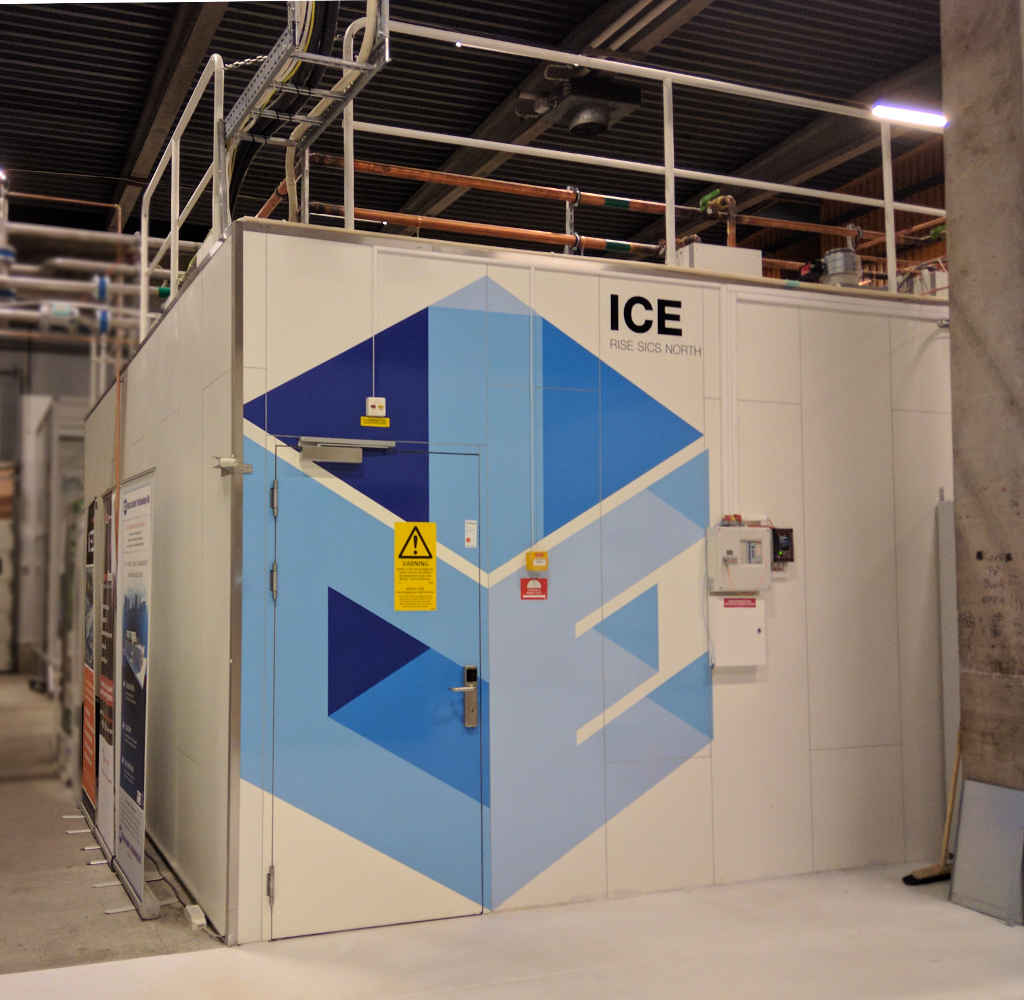
\includegraphics[width=0.55\linewidth]{pod1_exterior.jpg}
%\end{center}
%\caption{The exterior of data center module POD 1 at \gls{rsn}.}
%\end{figure}
